\documentclass[conference,onecolumn]{IEEEtran}
\IEEEoverridecommandlockouts
\usepackage{cite}
\usepackage{amsmath,amssymb,amsfonts}
\usepackage{algorithmic}
\usepackage{graphicx}
\usepackage{listings}
\usepackage{float}
\usepackage{textcomp}
\usepackage{gensymb}
\usepackage{xcolor}
\usepackage[spanish]{babel}
\def\BibTeX{{\rm B\kern-.05em{\sc i\kern-.025em b}\kern-.08em
    T\kern-.1667em\lower.7ex\hbox{E}\kern-.125emX}}

% --- Estilo de listados de codigo (borde verde, fondo blanco) ---
\definecolor{listinggreen}{RGB}{0,130,0}
\lstdefinestyle{tallerstyle}{backgroundcolor=\color{white},basicstyle=\ttfamily\footnotesize,breaklines=true,frame=single,rulecolor=\color{listinggreen},frameround=ffff,framesep=4pt,xleftmargin=6pt,xrightmargin=6pt,commentstyle=\color{gray},keywordstyle=\color{blue!70!black},stringstyle=\color{red!60!black},showstringspaces=false,columns=flexible,keepspaces=true,numbers=left,numberstyle=\tiny\color{gray}}
\lstset{style=tallerstyle}

\begin{document}

\title{Pr\'actica 4: Diversidad en transmisi\'on mediante SFBC (c\'odigo de Alamouti espacio-frecuencia) en un sistema OFDM conforme a LTE}

\author{\IEEEauthorblockN{Tyrone Miguel Novillo Bravo}
\IEEEauthorblockA{Facultad de Ingenier\'ia\\
Departamento de Telecomunicaciones\\
Universidad de Cuenca\\
tyrone.novillo@ucuenca.edu.ec}
\and
\IEEEauthorblockN{Freddy Eduardo L\'opez Padilla}
\IEEEauthorblockA{Facultad de Ingenier\'ia\\
Departamento de Telecomunicaciones\\
Universidad de Cuenca\\
freddy.lopez@ucuenca.edu.ec}}

\maketitle

\begin{abstract}
Este trabajo presenta la implementaci\'on y evaluaci\'on de la diversidad en transmisi\'on mediante SFBC (\textit{Space-Frequency Block Coding}), la variante espacio-frecuencia del c\'odigo de Alamouti que LTE emplea en el enlace descendente. A diferencia de la diversidad en recepci\'on, en la que el receptor combina varias copias de la se\~nal, SFBC traslada la complejidad al transmisor: emplea dos antenas y codifica cada par de s\'imbolos modulados $(s_0,s_1)$ sobre dos subportadoras OFDM adyacentes, transmitiendo $[s_0,\,s_1]$ por la primera antena y $[-s_1^{*},\,s_0^{*}]$ por la segunda. Con un \'unico receptor, un decodificador lineal ortogonal de baja complejidad recupera ambos s\'imbolos sin interferencia mutua y alcanza una diversidad de orden dos (orden cuatro con dos antenas de recepci\'on), la misma ganancia que el combinador de m\'axima relaci\'on (MRC) pero sin necesidad de m\'ultiples antenas en el terminal, a cambio de una penalizaci\'on cercana a $3$~dB por repartir la potencia entre las dos antenas. El simulador reutiliza \'integramente la cadena OFDM de las pr\'acticas anteriores (modulaciones QAM con codificaci\'on Gray, canal Pedestrian A con desvanecimiento de Rayleigh y ruido AWGN) y a\~nade \'unicamente el codificador y el decodificador SFBC. El desempe\~no se eval\'ua mediante un an\'alisis de Monte Carlo que estima las curvas de BER frente a SNR con intervalos de confianza al $95\%$ ($t$ de Student), comparando tres configuraciones ---sin diversidad ($1\times1$), SFBC $2\times1$ y SFBC $2\times2$--- cuyos \'ordenes de diversidad $1$, $2$ y $4$ se reflejan en pendientes crecientes. Toda la l\'ogica se implementa en Python y se expone mediante una interfaz web con pesta\~nas independientes.
\end{abstract}

\begin{IEEEkeywords}
SFBC, c\'odigo de Alamouti, diversidad en transmisi\'on, diversidad espacio-frecuencia, LTE, MISO, BER, Monte Carlo, OFDM, desvanecimiento de Rayleigh.
\end{IEEEkeywords}

\section*{Objetivos}

\textbf{Objetivo general:} Implementar y evaluar un esquema de diversidad en transmisi\'on SFBC (c\'odigo de Alamouti aplicado en el dominio espacio-frecuencia) sobre la cadena OFDM de las pr\'acticas anteriores, y verificar que proporciona ganancia de diversidad ---reducci\'on de la BER frente a SNR--- equivalente a la diversidad en recepci\'on pero ubicando las antenas en el transmisor.

\textbf{Objetivos espec\'ificos:}
\begin{itemize}
    \item Implementar el codificador SFBC de Alamouti sobre pares de subportadoras adyacentes y su decodificador ortogonal de m\'axima verosimilitud.
    \item Integrar el esquema en la misma cadena de transmisi\'on, canal y recepci\'on que OFDM (canal Pedestrian A, AWGN), reutilizando los m\'odulos comunes.
    \item Transmitir im\'agenes con las configuraciones $2\times1$ y $2\times2$ y comparar la calidad recuperada frente al caso sin diversidad.
    \item Caracterizar la ganancia de diversidad mediante curvas de BER frente a SNR (Monte Carlo) para las configuraciones $1\times1$, $2\times1$ y $2\times2$, verificando los \'ordenes de diversidad $1$, $2$ y $4$.
\end{itemize}

\section{Introducci\'on}

El desvanecimiento multitrayecto es la principal limitaci\'on de los canales m\'oviles: la se\~nal recibida sufre desvanecimientos profundos cuando las componentes que llegan por distintos caminos se combinan destructivamente, lo que dispara la tasa de error de bit (BER). La diversidad es la t\'ecnica fundamental para combatirlo, ya que entrega al receptor varias r\'eplicas de la se\~nal afectadas por desvanecimientos independientes, de modo que la probabilidad de que todas se desvanezcan a la vez disminuye exponencialmente con el n\'umero de r\'eplicas \cite{goldsmith2005wireless,rappaport2002}. La pr\'actica anterior abord\'o la diversidad en \emph{recepci\'on}, en la que el receptor combina las se\~nales de varias antenas con MRC; la presente aborda la diversidad en \emph{transmisi\'on}, en la que la diversidad se genera desde m\'ultiples antenas en el transmisor.

La diversidad en transmisi\'on es especialmente atractiva en el enlace descendente celular, donde resulta econ\'omico instalar varias antenas en la estaci\'on base pero no en el terminal m\'ovil, limitado por tama\~no, costo y bater\'ia. El reto es que, a diferencia del receptor con MRC, el transmisor no conoce el canal y no puede ponderar coherentemente las antenas. Alamouti resolvi\'o este problema en 1998 con un c\'odigo de bloque espacio-tiempo notablemente simple para dos antenas que logra diversidad de orden dos con un decodificador lineal y sin conocimiento del canal en el transmisor \cite{alamouti1998}. Aplicado sobre los s\'imbolos de tiempo consecutivos se denomina STBC; aplicado sobre subportadoras de frecuencia adyacentes de un s\'imbolo OFDM se denomina SFBC, que es la forma adoptada por LTE en el enlace descendente \cite{sesia2011lte,3gpp36211}. Este trabajo extiende el simulador OFDM para incorporar SFBC, reutilizando toda la cadena com\'un y a\~nadiendo \'unicamente el par codificador/decodificador de Alamouti, y verifica la ganancia de diversidad mediante un an\'alisis de Monte Carlo que compara las configuraciones $1\times1$, $2\times1$ y $2\times2$.

\section{Marco te\'orico}

\subsection{Diversidad en transmisi\'on y el c\'odigo de Alamouti}

El c\'odigo de Alamouti es un c\'odigo de bloque espacio-tiempo (o espacio-frecuencia) ortogonal de tasa unitaria para dos antenas de transmisi\'on. La idea central es transmitir dos s\'imbolos $(s_0,s_1)$ en dos \emph{recursos} ortogonales (dos instantes de tiempo en STBC, o dos subportadoras en SFBC) con una estructura conjugada que permite separarlos en el receptor mediante operaciones lineales \cite{alamouti1998,tarokh1999}. Su importancia radica en que alcanza el mismo orden de diversidad que un receptor MRC con el mismo n\'umero de ramas, pero trasladando las antenas y la complejidad de codificaci\'on al transmisor, sin requerir conocimiento del canal en \'el.

\subsection{SFBC: el c\'odigo de Alamouti en el dominio espacio-frecuencia}

En SFBC el bloque de s\'imbolos modulados se agrupa en parejas $(s_0,s_1)$ que se asignan a dos subportadoras adyacentes $k$ y $k{+}1$ de un mismo s\'imbolo OFDM. Las dos antenas transmiten simult\'aneamente seg\'un la matriz de codificaci\'on
\begin{equation}
\mathbf{S}=\frac{1}{\sqrt{2}}
\begin{bmatrix} s_0 & s_1 \\[2pt] -s_1^{*} & s_0^{*} \end{bmatrix},
\label{eq:matriz}
\end{equation}
donde las filas son las antenas (1 y 2) y las columnas las subportadoras ($k$ y $k{+}1$). Es decir, la antena~1 env\'ia $[s_0,\,s_1]$ y la antena~2 env\'ia $[-s_1^{*},\,s_0^{*}]$. El factor $1/\sqrt{2}$ reparte la potencia entre las dos antenas para mantener constante la potencia total radiada respecto a una transmisi\'on de una sola antena.

Llamando $h_1$ y $h_2$ a las respuestas del canal de cada antena de transmisi\'on hacia el receptor, y suponiendo que el canal var\'ia lentamente en frecuencia de modo que es pr\'acticamente igual en las dos subportadoras del par ($H_1[k]\!\approx\!H_1[k{+}1]\!\equiv\!h_1$ y $H_2[k]\!\approx\!H_2[k{+}1]\!\equiv\!h_2$), las muestras recibidas en una antena son
\begin{equation}
r_0 = h_1 s_0 - h_2 s_1^{*} + n_0, \qquad
r_1 = h_1 s_1 + h_2 s_0^{*} + n_1,
\label{eq:recibido}
\end{equation}
donde $n_0$ y $n_1$ es el ruido AWGN en cada subportadora (se omite el factor $1/\sqrt{2}$ por claridad).

\subsection{Decodificador ortogonal y orden de diversidad}

Conocido el canal en el receptor, el decodificador de Alamouti recombina las dos muestras de \eqref{eq:recibido} como
\begin{equation}
\hat{s}_0 = h_1^{*} r_0 + h_2 r_1^{*}, \qquad
\hat{s}_1 = h_1^{*} r_1 - h_2 r_0^{*}.
\label{eq:decod}
\end{equation}
Sustituyendo \eqref{eq:recibido} en \eqref{eq:decod}, los t\'erminos cruzados se cancelan gracias a la ortogonalidad de la matriz \eqref{eq:matriz} y se obtiene
\begin{equation}
\hat{s}_0 = \big(|h_1|^{2}+|h_2|^{2}\big)\,s_0 + \tilde{n}_0, \qquad
\hat{s}_1 = \big(|h_1|^{2}+|h_2|^{2}\big)\,s_1 + \tilde{n}_1,
\label{eq:estimado}
\end{equation}
es decir, cada s\'imbolo se recupera \emph{sin interferencia} del otro, escalado por la suma de las ganancias de ambos canales. La forma de \eqref{eq:estimado} es id\'entica a la del combinador MRC: el s\'imbolo se beneficia de la energ\'ia de los dos trayectos independientes, por lo que el sistema alcanza \textbf{diversidad de orden 2} con una sola antena de recepci\'on. Si el receptor dispone de $N_{rx}$ antenas, se suman los numeradores y denominadores de \eqref{eq:decod}--\eqref{eq:estimado} sobre todas ellas y el orden de diversidad asciende a $2N_{rx}$ ($2\times2\Rightarrow$ orden $4$). En r\'egimen asint\'otico (SNR alta), la BER de un sistema de orden de diversidad $d$ decae como
\begin{equation}
\mathrm{BER}\;\propto\;\mathrm{SNR}^{-d},
\label{eq:diversidad}
\end{equation}
lo que se traduce en una pendiente de $-10d$~dB por d\'ecada en escala logar\'itmica: a mayor orden, mayor pendiente de ca\'ida.

\subsection{Reparto de potencia: la penalizaci\'on respecto a MRC}

El c\'odigo de Alamouti $2\times1$ y el MRC $1\times2$ tienen el mismo orden de diversidad (2), pero no son id\'enticos. En MRC el receptor recibe la potencia completa por cada una de sus dos antenas, mientras que en SFBC el transmisor debe \emph{repartir} su potencia entre las dos antenas (factor $1/\sqrt{2}$ en \eqref{eq:matriz}) para no radiar el doble de potencia total. Esa diferencia se traduce en una penalizaci\'on de aproximadamente $3$~dB de SFBC $2\times1$ frente a MRC $1\times2$ a igualdad de BER y de potencia total transmitida \cite{alamouti1998}. Es el precio de mover la diversidad al transmisor; a cambio, el terminal m\'ovil conserva una sola antena y una recepci\'on sencilla.

\subsection{Componentes reutilizados de la cadena OFDM}

El resto de la cadena es id\'entico al de las pr\'acticas anteriores y se reutiliza sin cambios: las modulaciones QPSK, 16-QAM y 64-QAM con codificaci\'on Gray y energ\'ia media unitaria \cite{proakis2008digital}; el canal Pedestrian A (ITU-R M.1225) de cuatro taps con desvanecimiento de Rayleigh (Tabla~\ref{tab:pedA}), generado de forma independiente para cada enlace antena-transmisora$\rightarrow$antena-receptora \cite{ituR1225,rappaport2002}; el ruido AWGN calibrado por SNR; y la validaci\'on estad\'istica mediante Monte Carlo con intervalos de confianza basados en la distribuci\'on $t$ de Student \cite{montgomery2011}. El conocimiento del canal en el receptor es perfecto (\textit{genie}), como en el resto del simulador. La suposici\'on de canal aproximadamente constante en subportadoras adyacentes que requiere \eqref{eq:recibido} se cumple con holgura: el canal Pedestrian A tiene un ancho de banda de coherencia del orden de $390$~kHz, muy superior al espaciamiento de $15$~kHz entre subportadoras \cite{cho2010mimo}.

\begin{table}[H]
    \renewcommand{\arraystretch}{1.2}
    \caption{Perfil potencia-retardo del modelo Pedestrian A \cite{ituR1225}.}
    \label{tab:pedA}
    \centering
    \begin{tabular}{ccc}
        \hline
        \textbf{Tap} & \textbf{Retardo (ns)} & \textbf{Potencia (dB)} \\
        \hline
        1 & 0   & 0       \\
        2 & 110 & -9{,}7  \\
        3 & 190 & -19{,}2 \\
        4 & 410 & -22{,}8 \\
        \hline
    \end{tabular}
\end{table}

\section{Metodolog\'ia -- Desarrollo de la pr\'actica}

Toda la l\'ogica de procesamiento se mantiene en el m\'odulo \'unico \texttt{app.py} (Python con \texttt{numpy}, \texttt{scipy} y \texttt{Pillow}), expuesto mediante una interfaz web Flask. SFBC se a\~nadi\'o como una funci\'on de cadena propia, \texttt{cadena\_tx\_sfbc\_rx}, hermana de la cadena OFDM/SC-FDM, que reutiliza los m\'odulos comunes (modulaciones QAM, canal, ruido, IFFT/FFT con prefijo c\'iclico) y solo implementa lo espec\'ifico del esquema: el codificador y el decodificador de Alamouti.

\subsection{Mapeo por pares de subportadoras}

A diferencia de OFDM, SFBC no intercala tonos piloto: emplea \emph{todas} las subportadoras de datos agrup\'andolas en pares contiguos $(2j,\,2j{+}1)$, de modo que el n\'umero de parejas Alamouti por s\'imbolo OFDM es $N_{par}=N_{SC}/2$. Esta decisi\'on ---an\'aloga a la de SC-FDM y coherente con LTE, donde las se\~nales de referencia van en recursos dedicados--- garantiza que los dos elementos de cada par sean f\'isicamente adyacentes en frecuencia, condici\'on necesaria para que se cumpla $h_1[k]\!\approx\!h_1[k{+}1]$ en el decodificador. Los s\'imbolos pares e impares de cada bloque se separan con $\texttt{s0}=\texttt{bloque[0::2]}$ y $\texttt{s1}=\texttt{bloque[1::2]}$.

\subsection{Codificador SFBC}

El codificador construye dos rejillas de subportadoras, una por antena, siguiendo la matriz \eqref{eq:matriz}. El factor \texttt{esc}$=1/\sqrt{2}$ reparte la potencia entre ambas antenas.

\begin{lstlisting}[language=Python]
esc = 1/np.sqrt(2)                      # reparto de potencia entre las 2 antenas
x1[0::2][:n_par] = esc * s0             # antena 1, subportadora k   ->  s0
x1[1::2][:n_par] = esc * s1             # antena 1, subportadora k+1 ->  s1
x2[0::2][:n_par] = esc * (-np.conj(s1)) # antena 2, subportadora k   -> -s1*
x2[1::2][:n_par] = esc * ( np.conj(s0)) # antena 2, subportadora k+1 ->  s0*
\end{lstlisting}

\subsection{Canal independiente por antena y decodificador ortogonal}

Cada antena de transmisi\'on atraviesa un canal Pedestrian A independiente ($H_1$, $H_2$); las dos contribuciones se suman en el aire y se les a\~nade el ruido AWGN una sola vez. En el receptor se separan las subportadoras pares ($r_0$) e impares ($r_1$) y se aplican las ecuaciones \eqref{eq:decod}, acumulando sobre las $N_{rx}$ antenas de recepci\'on.

\begin{lstlisting}[language=Python]
for r in range(n_rx):
    H1 = generar_canal_pedestrian_a(n_fft, fs, indices_fft, rng)   # TX1 -> RX
    H2 = generar_canal_pedestrian_a(n_fft, fs, indices_fft, rng)   # TX2 -> RX
    senal1, _ = modulacion_ofdm(x1 * H1, n_fft, n_cp)
    senal2, _ = modulacion_ofdm(x2 * H2, n_fft, n_cp)
    senal_rx = agregar_ruido_awgn(senal1 + senal2, snr_db, rng)    # suma + AWGN
    rejilla_rx = demodulacion_ofdm(senal_rx, indices_fft, n_fft, n_cp, n_sc)
    r0, r1 = rejilla_rx[0::2][:n_par], rejilla_rx[1::2][:n_par]
    h1, h2 = H1[0::2][:n_par], H2[0::2][:n_par]
    num0 += np.conj(h1)*r0 + h2*np.conj(r1)    # estimador de s0
    num1 += np.conj(h1)*r1 - h2*np.conj(r0)    # estimador de s1
    den  += np.abs(h1)**2 + np.abs(h2)**2
s0_est = (num0 / (den + 1e-12)) / esc          # /esc restituye la escala unitaria
s1_est = (num1 / (den + 1e-12)) / esc
\end{lstlisting}

La divisi\'on final por \texttt{esc} restituye la constelaci\'on a su escala de energ\'ia unitaria tras la normalizaci\'on \eqref{eq:estimado} por \texttt{den}$=|h_1|^2+|h_2|^2$, paso imprescindible para que el demapeador de 16-QAM y 64-QAM aplique las regiones de decisi\'on correctas. La rama sin diversidad ($1\times1$) reutiliza la misma estructura con una sola antena y ecualizaci\'on Zero-Forcing, lo que permite comparar las tres configuraciones bajo id\'entica carga \'util.

\subsection{Endpoints e interfaz}

La l\'ogica se expone en dos \emph{endpoints}: \texttt{simular\_sfbc} transmite la imagen cargada con la configuraci\'on elegida ($2\times1$ o $2\times2$) y, sobre los mismos bits, una cadena $1\times1$ de referencia, devolviendo ambas constelaciones para la comparaci\'on ``sin diversidad vs SFBC''; \texttt{montecarlo\_sfbc} ejecuta el barrido de BER frente a SNR con $8$ corridas por punto e intervalos de confianza al $95\%$, calculando una curva por cada configuraci\'on de la lista $\{1\times1,\,2\times1,\,2\times2\}$. La interfaz a\~nade una pesta\~na ``Diversidad TX (SFBC)'' con un selector de configuraci\'on y el resto de controles compartidos. La Fig.~\ref{fig:diagrama} resume el diagrama de bloques de la cadena, en el que se resaltan el codificador y el decodificador SFBC.

\begin{figure}[H]
\centering
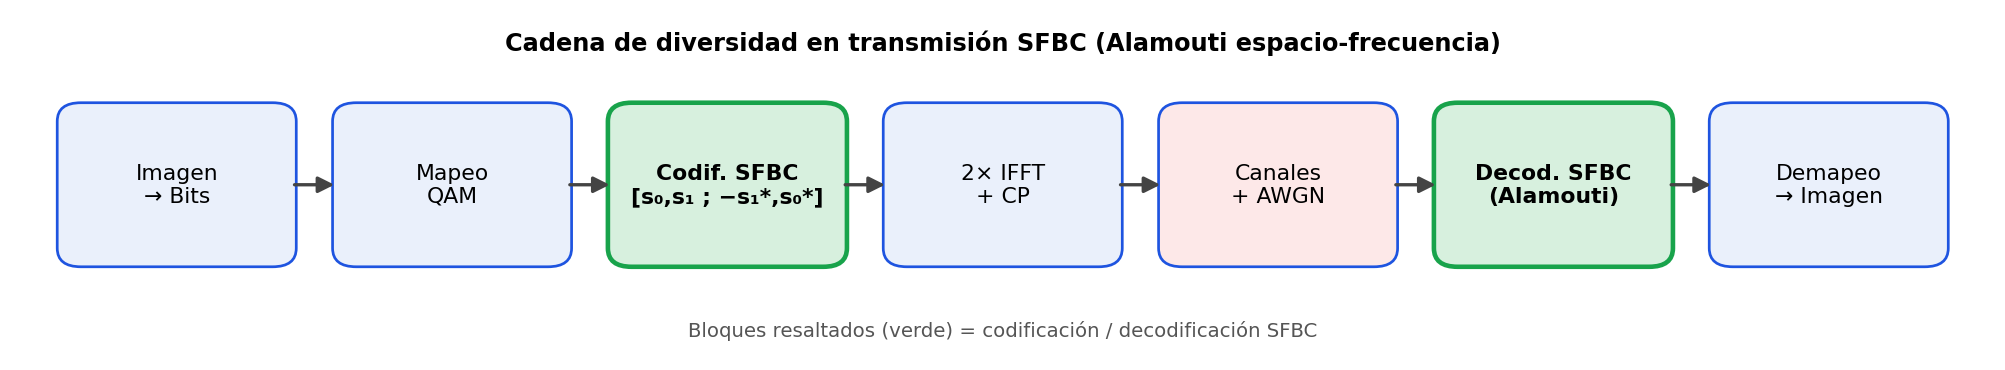
\includegraphics[width=0.95\textwidth]{img/diagrama_sfbc.png}
\caption{Diagrama de bloques de la cadena SFBC; se resaltan el codificador de Alamouti $[s_0,s_1;\,-s_1^{*},s_0^{*}]$ y el decodificador ortogonal, los bloques que la diferencian del transmisor OFDM de una sola antena.}
\label{fig:diagrama}
\end{figure}

\section{Evaluaci\'on -- An\'alisis de resultados}

En esta secci\'on se analizan los resultados del simulador SFBC. Se describen la interfaz y los par\'ametros de configuraci\'on; se examinan transmisiones de imagen con las configuraciones $2\times1$ y $2\times2$; se inspecciona la constelaci\'on recibida sin diversidad frente a SFBC; y se caracteriza la ganancia de diversidad mediante las curvas de BER frente a SNR obtenidas por Monte Carlo, que constituyen el resultado central de la pr\'actica. La configuraci\'on empleada es $BW{=}5$~MHz, $\Delta f{=}15$~kHz y CP normal.

\subsection{Interfaz y par\'ametros de configuraci\'on}

La Fig.~\ref{fig:params} resume los par\'ametros derivados para la configuraci\'on empleada: $N_{SC}=300$ subportadoras, $N_{FFT}=512$, $f_s=7{,}680$~MHz y $N_{CP}=36$ muestras. La diferencia respecto a OFDM aparece en la organizaci\'on de las subportadoras: SFBC las agrupa en $N_{par}=N_{SC}/2=150$ parejas Alamouti y no intercala pilotos, por lo que toda la rejilla transporta datos. La duraci\'on de cada s\'imbolo OFDM es de $71{,}35~\mu$s.

\begin{figure}[H]
\centering
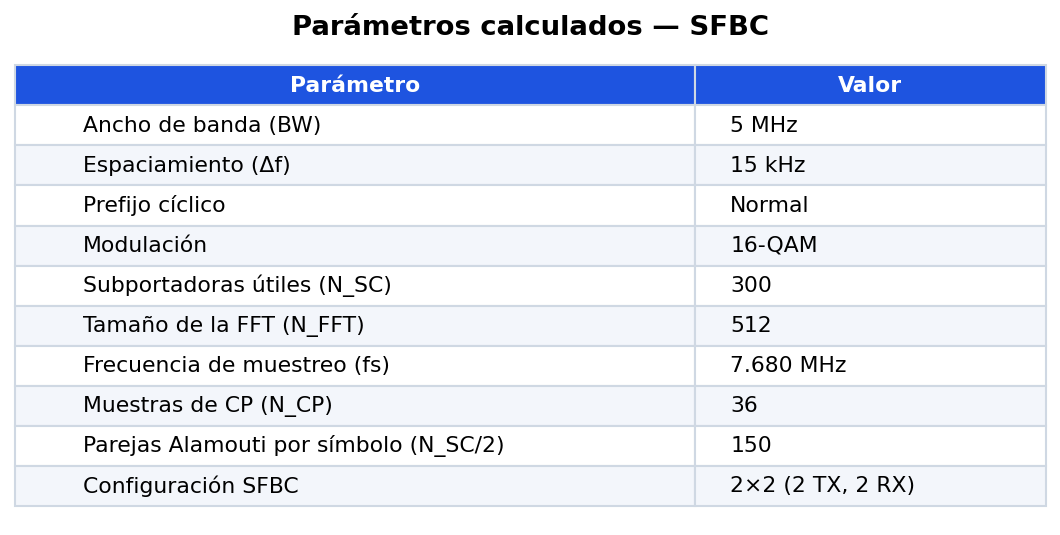
\includegraphics[width=0.95\textwidth]{img/params_sfbc.png}
\caption{Par\'ametros calculados para SFBC ($BW{=}5$~MHz, $\Delta f{=}15$~kHz, CP normal): $N_{SC}{=}300$, $N_{FFT}{=}512$, $150$ parejas Alamouti por s\'imbolo y configuraci\'on seleccionada.}
\label{fig:params}
\end{figure}

\subsection{Transmisi\'on de im\'agenes con SFBC}

Se transmiti\'o la misma imagen de prueba ($256\times256$ p\'ixeles) con 16-QAM y SNR de $12$~dB en las dos configuraciones, resumidas en la Tabla~\ref{tab:sims}. Con SFBC $2\times1$ (Fig.~\ref{fig:sim2x1}) la imagen se recupera con un moteado moderado y una BER de $1{,}1\times10^{-2}$, frente a la BER de $1{,}9\times10^{-2}$ del caso sin diversidad ($1\times1$) en las mismas condiciones. Con SFBC $2\times2$ (Fig.~\ref{fig:sim2x2}) la imagen es pr\'acticamente id\'entica a la original y la BER baja a $1{,}4\times10^{-3}$, m\'as de un orden de magnitud por debajo del caso $1\times1$, lo que evidencia el efecto de la diversidad de orden cuatro a igualdad de SNR.

\begin{table}[H]
\centering
\caption{Resultados de las transmisiones de imagen con SFBC (16-QAM, SNR${=}12$~dB).}
\label{tab:sims}
\begin{tabular}{|l|c|c|c|}
\hline
\textbf{Configuraci\'on} & \textbf{Orden div.} & \textbf{BER} & \textbf{S\'imb. OFDM} \\
\hline
Sin diversidad ($1\times1$) & $1$ & $1{,}9\times10^{-2}$ & $1311$ \\
SFBC $2\times1$             & $2$ & $1{,}1\times10^{-2}$ & $1311$ \\
SFBC $2\times2$             & $4$ & $1{,}4\times10^{-3}$ & $1311$ \\
\hline
\end{tabular}
\end{table}

\begin{figure}[H]
\centering
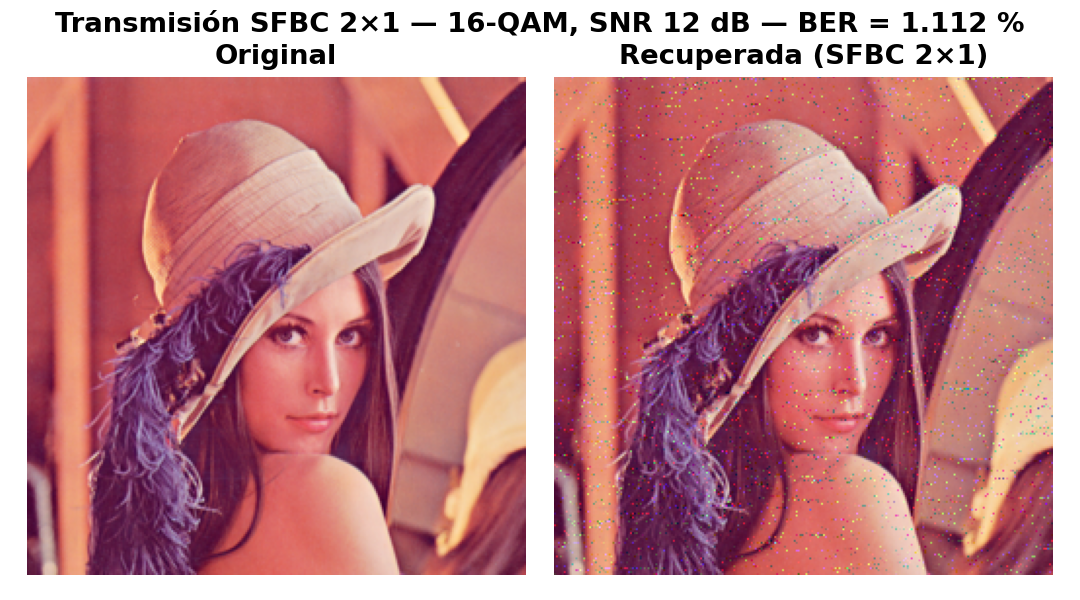
\includegraphics[width=0.6\textwidth]{img/sim_2x1_sfbc.png}
\caption{Transmisi\'on SFBC $2\times1$ con 16-QAM y SNR${=}12$~dB. La imagen recuperada presenta un moteado moderado (BER ${=}1{,}1\times10^{-2}$).}
\label{fig:sim2x1}
\end{figure}

\begin{figure}[H]
\centering
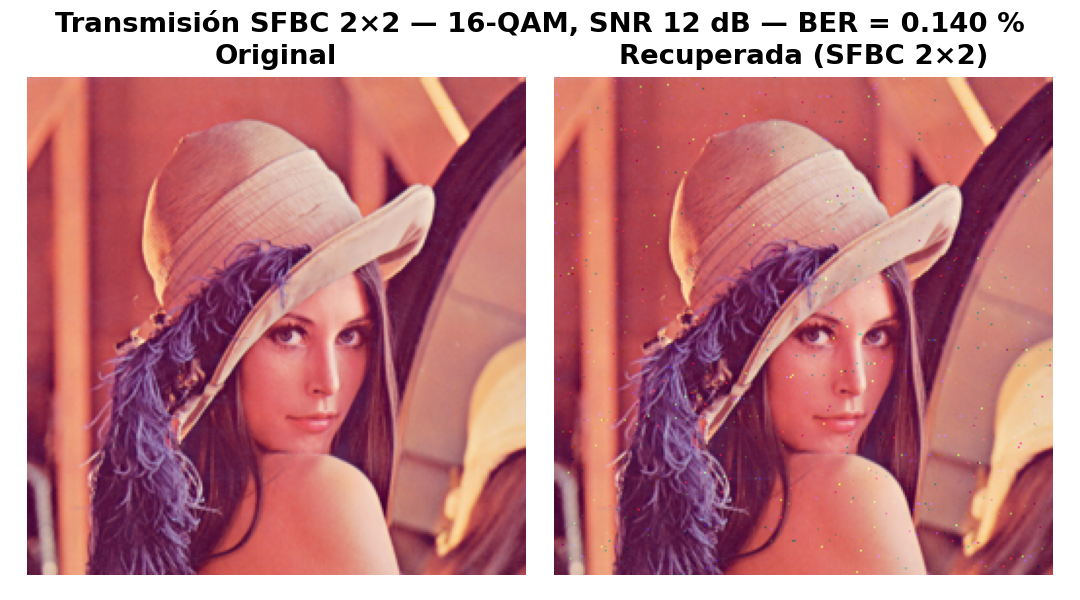
\includegraphics[width=0.6\textwidth]{img/sim_2x2_sfbc.png}
\caption{Transmisi\'on SFBC $2\times2$ con 16-QAM y SNR${=}12$~dB. La imagen recuperada es pr\'acticamente id\'entica a la original (BER ${=}1{,}4\times10^{-3}$).}
\label{fig:sim2x2}
\end{figure}

\subsection{Constelaci\'on recibida: sin diversidad frente a SFBC}

La Fig.~\ref{fig:const} compara la constelaci\'on de 16-QAM recibida sin diversidad ($1\times1$, izquierda) y con SFBC (derecha). En el caso sin diversidad los s\'imbolos aparecen muy dispersos debido a los desvanecimientos profundos del canal Pedestrian A, que la ecualizaci\'on Zero-Forcing de una sola antena no puede corregir. Con SFBC la nube se compacta notablemente en torno a las posiciones ideales de la ret\'icula, pues el decodificador de Alamouti combina la energ\'ia de los dos trayectos independientes seg\'un \eqref{eq:estimado}, reduciendo la probabilidad de un desvanecimiento simult\'aneo. Esta compactaci\'on es la manifestaci\'on visual directa de la ganancia de diversidad.

\begin{figure}[H]
\centering
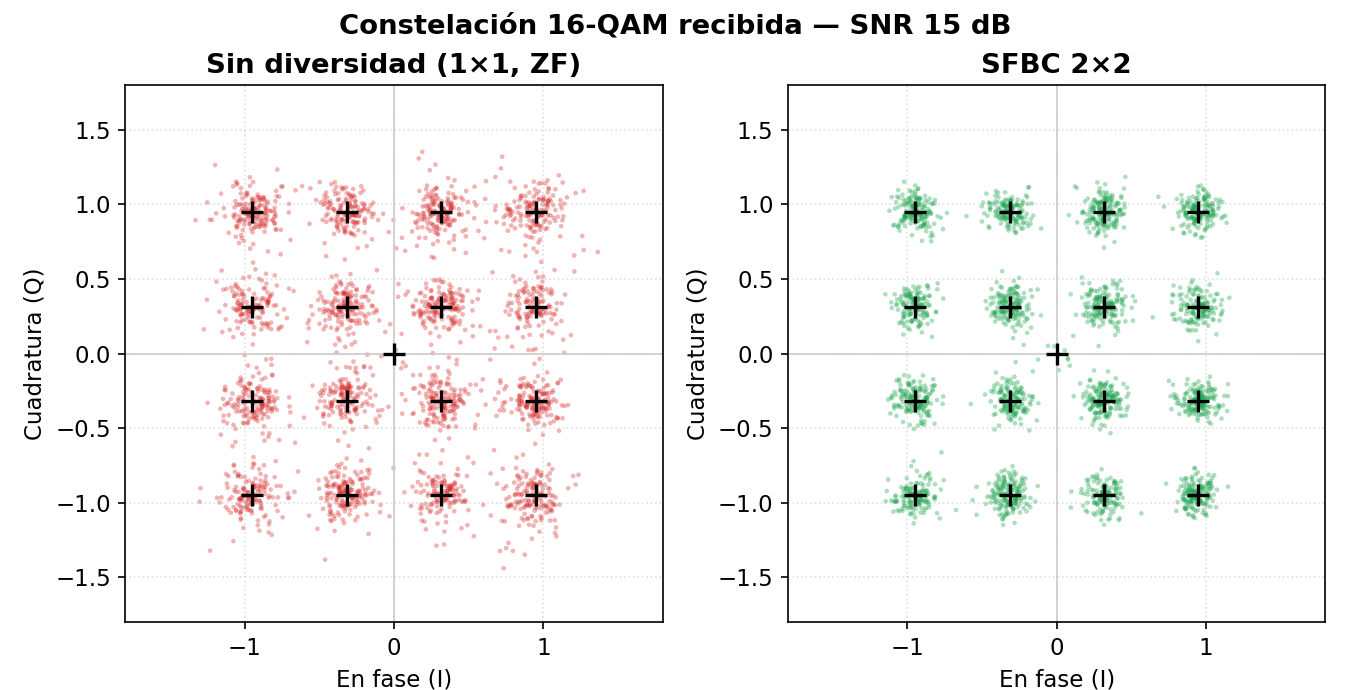
\includegraphics[width=0.95\textwidth]{img/constelacion_sfbc.png}
\caption{Constelaci\'on de 16-QAM recibida: sin diversidad ($1\times1$, izquierda, dispersa) frente a SFBC (derecha, compacta). La diversidad en transmisi\'on agrupa los s\'imbolos en torno a la ret\'icula ideal.}
\label{fig:const}
\end{figure}

\subsection{Curvas BER frente a SNR (Monte Carlo): resultado central}

La Fig.~\ref{fig:montecarlo} superpone las tres curvas de BER frente a SNR obtenidas con $8$ corridas independientes por punto e intervalos de confianza al $95\%$ ($t$ de Student) para 16-QAM: sin diversidad ($1\times1$), SFBC $2\times1$ y SFBC $2\times2$. El resultado reproduce el comportamiento can\'onico descrito por Alamouti \cite{alamouti1998}: las tres curvas exhiben \emph{pendientes claramente distintas}, correspondientes a los \'ordenes de diversidad $1$, $2$ y $4$ de \eqref{eq:diversidad}. La Tabla~\ref{tab:ber} recoge valores representativos: a $15$~dB la BER pasa de $7{,}1\times10^{-3}$ sin diversidad a $1{,}5\times10^{-3}$ con SFBC $2\times1$ y a $5{,}3\times10^{-5}$ con SFBC $2\times2$, y la separaci\'on entre las curvas se ensancha al aumentar la SNR, tal como predice la diferencia de pendientes. Se verifica adem\'as que SFBC $2\times1$, pese a compartir el orden de diversidad $2$ con un receptor MRC $1\times2$, queda unos $2$ a $3$~dB por encima de \'este a igualdad de BER, lo que corresponde a la penalizaci\'on por el reparto de potencia entre las dos antenas transmisoras.

\begin{table}[H]
\centering
\caption{BER frente a SNR (Monte Carlo, 16-QAM) para las tres configuraciones.}
\label{tab:ber}
\begin{tabular}{|c|c|c|c|}
\hline
\textbf{SNR (dB)} & \textbf{$1\times1$} & \textbf{SFBC $2\times1$} & \textbf{SFBC $2\times2$} \\
\hline
$6$  & $1{,}1\times10^{-1}$ & $9{,}6\times10^{-2}$ & $4{,}8\times10^{-2}$ \\
$9$  & $5{,}2\times10^{-2}$ & $4{,}3\times10^{-2}$ & $1{,}3\times10^{-2}$ \\
$12$ & $2{,}2\times10^{-2}$ & $1{,}3\times10^{-2}$ & $1{,}8\times10^{-3}$ \\
$15$ & $7{,}1\times10^{-3}$ & $1{,}5\times10^{-3}$ & $5{,}3\times10^{-5}$ \\
$18$ & $2{,}6\times10^{-3}$ & $2{,}8\times10^{-4}$ & $<10^{-5}$ \\
\hline
\end{tabular}
\end{table}

\begin{figure}[H]
\centering
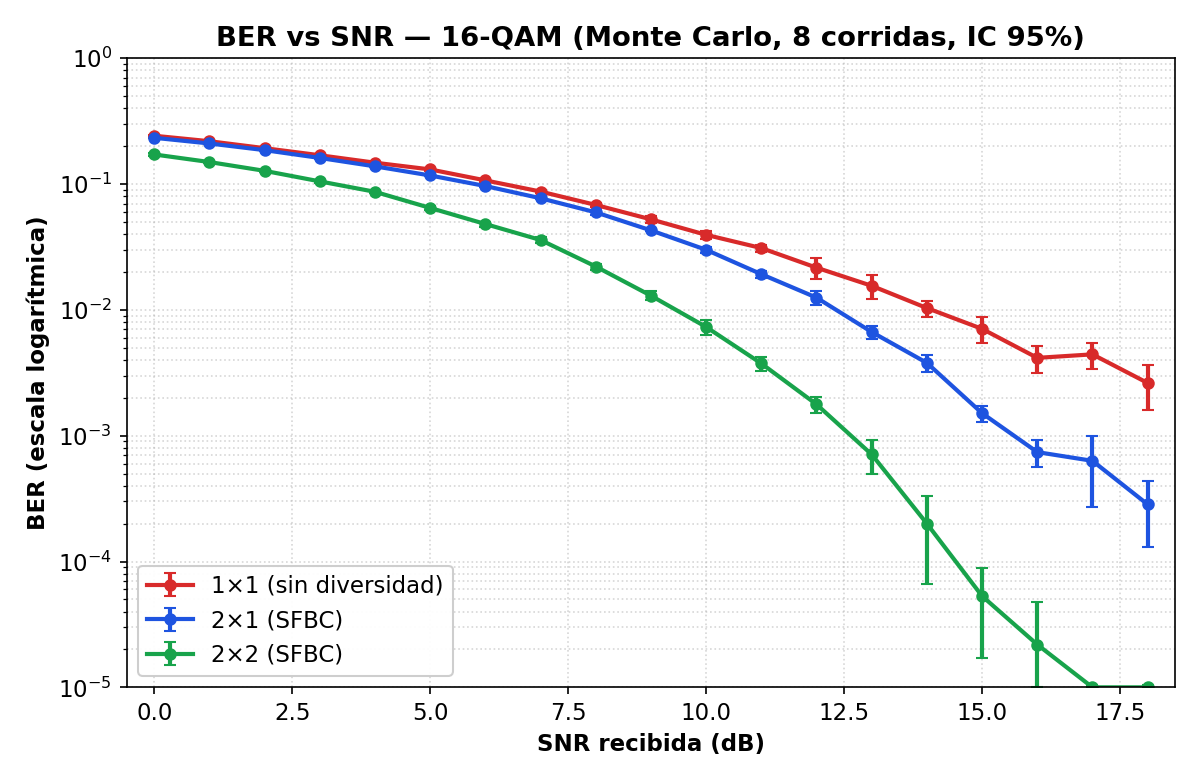
\includegraphics[width=0.9\textwidth]{img/montecarlo_sfbc.png}
\caption{BER frente a SNR (16-QAM): sin diversidad ($1\times1$), SFBC $2\times1$ y SFBC $2\times2$, Monte Carlo con $8$ corridas por punto e IC al $95\%$. Las pendientes crecientes corresponden a los \'ordenes de diversidad $1$, $2$ y $4$.}
\label{fig:montecarlo}
\end{figure}

\section{Conclusiones}

Se implement\'o y evalu\'o un esquema de diversidad en transmisi\'on SFBC (c\'odigo de Alamouti espacio-frecuencia) reutilizando \'integramente la cadena OFDM de las pr\'acticas anteriores. La incorporaci\'on requiri\'o \'unicamente dos elementos espec\'ificos ---el codificador de Alamouti sobre pares de subportadoras adyacentes y su decodificador ortogonal con compensaci\'on del reparto de potencia---, lo que confirma que SFBC se integra de forma natural sobre OFDM aprovechando que el canal es aproximadamente constante en subportadoras contiguas. La segmentaci\'on previa del c\'odigo en m\'odulos comunes y espec\'ificos facilit\'o esta extensi\'on sin mezclar la l\'ogica de las distintas pr\'acticas.

Los resultados verifican el objetivo de la pr\'actica. El an\'alisis de Monte Carlo mostr\'o que las curvas de BER frente a SNR de las configuraciones $1\times1$, $2\times1$ y $2\times2$ presentan pendientes crecientes acordes con los \'ordenes de diversidad $1$, $2$ y $4$, y que la separaci\'on entre ellas se ensancha con la SNR, evidenciando una \emph{ganancia de diversidad} an\'aloga a la obtenida en recepci\'on pero generada desde el transmisor. La comparaci\'on de las transmisiones de imagen y de las constelaciones confirm\'o visualmente esta mejora: la nube de s\'imbolos se compacta y la imagen recuperada gana calidad al a\~nadir diversidad. Se observ\'o, adem\'as, la penalizaci\'on de $2$ a $3$~dB de SFBC $2\times1$ respecto a MRC $1\times2$, inherente al reparto de potencia entre las antenas transmisoras. Esta capacidad de obtener diversidad sin exigir m\'ultiples antenas en el terminal es precisamente la raz\'on por la que LTE adopta SFBC en el enlace descendente: traslada el costo de la diversidad a la estaci\'on base, donde resulta asumible.

\bibliographystyle{IEEEtran}
\bibliography{referencias}

\clearpage
\onecolumn
\newpage
\section*{Anexos}

\begin{figure}[H]
    \centering
    
\includegraphics[width=0.22\textwidth]{img/qr_sitio.png}
    \caption{C\'odigo QR del simulador desplegado: \texttt{https://ofdm.tesisucuenca.com}}
    \label{fig:qrsitio}
\end{figure}

\begin{figure}[H]
    \centering
    
\includegraphics[width=0.22\textwidth]{img/qr_repo.png}
    \caption{C\'odigo QR del repositorio del proyecto: \texttt{https://github.com/thyron001/ofdm}}
    \label{fig:qrrepo}
\end{figure}

\end{document}
